\documentclass[Interploate_hadwritten_Digits.tex]{subfiles}

\begin{document}
	\subsection{Erkennen von Ziffern}
	Das Neuronale Netz zum Erkennen der Ziffern erreicht nach 100 Trainingsiterationen im Normalfall eine Genauigkeit von circa 88\% (siehe Abbildung \ref{fig:hist_network_accuracy}) mit einigen Ausreissern welche darunter befinden. Auch lassen sich in den Konfusionsmatrizen keine grossen Fehltritte erkennen, erhöhte Fehlerwerte lassen sich lediglich bei ähnlichen Ziffern (wie 3 \& 5 oder 4 \& 9) erkennen. Alle Konfusionsmatrizen sind im Anhang (Kapitel \ref{sec:apendix_konfusion_network}) zu finden.
	\begin{Figure}
		\centering
		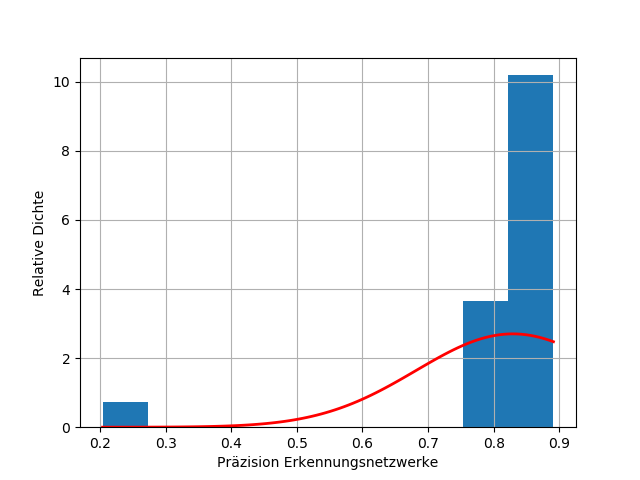
\includegraphics[width=\linewidth]{img/results/histogram_network_accuracy.png}
		\captionof{figure}{Präzision des Neuronalen Neztes}
		\label{fig:hist_network_accuracy}
	\end{Figure}

	\subsection{Netzwerk Komprimierung}
	\label{sec:results_compression}
	Die Komprimierung des Netzwerkes gemäss Kapitel \ref{sec:method_compress} in eine Matrix führt zu einem starken Qualitätsverlust der Vorhersagen. Der grosse Teil der komprimierten Netze erreicht mit einer Trefferquote von 30\%, wie in Abbildung \ref{fig:hist_compressed_network_accuracy} zu erkennen ist. Es sind Ausreisser zu erkennen, deren Werte liegen aber mit einer Trefferquote von maximal 45\% weit entfernt von den Werten der unkomprimierten Netze.
	\begin{Figure}
		\centering
		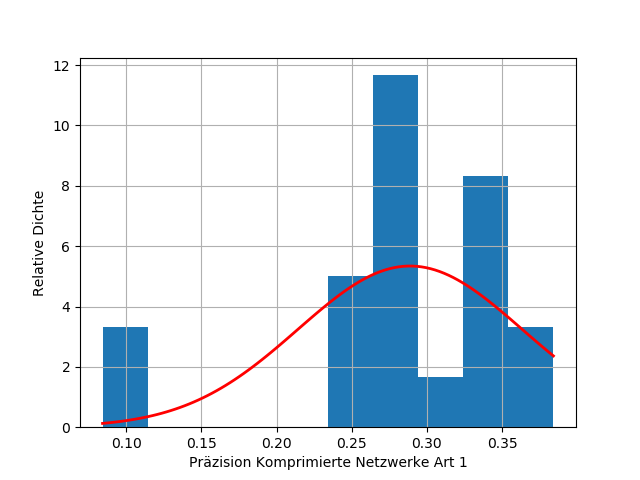
\includegraphics[width=\linewidth]{img/results/histogram_compressed_network_accuracy.png}
		\captionof{figure}{Präzision des komprimierten Neuronalen Neztes Methode 1}
		\label{fig:hist_compressed_network_accuracy}
	\end{Figure}

	In der zweiten Methode der Komprimierung, bei welcher die Aktivierungsfunktion nur auf das Resultat der Vorhersage anwendet, ist ebenfalls eine Verschlechterung der Werte zu erkennen. Diese ist sogar noch stärker. So verteilen sich die Werte gemäss Abbildung \ref{fig:hist_compressed_network_v2_accuracy} zwischen 10\% und 20\%. Somit liegt die Untergrenze bei Werten, welche durch eine zufällige Klassifikation erreicht werden könnte.
	\begin{Figure}
		\centering
		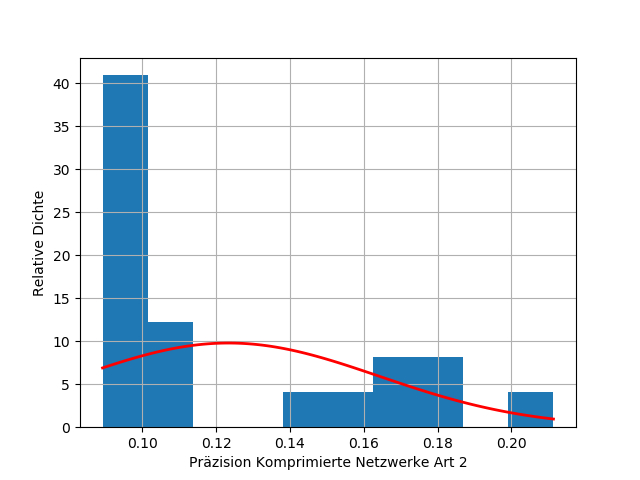
\includegraphics[width=\linewidth]{img/results/histogram_compressed_network_v2_accuracy.png}
		\captionof{figure}{Präzision des komprimierten Neuronalen Neztes Methode 2}
		\label{fig:hist_compressed_network_v2_accuracy}
	\end{Figure}

	Die Invertierung mit mehreren erreicht die selben Werte wie die ursprüngliche Version. Dies ist in der Abbildung \ref{fig:hist_inverted_network_accuracy} zu erkennen.
	\begin{Figure}
		\centering
		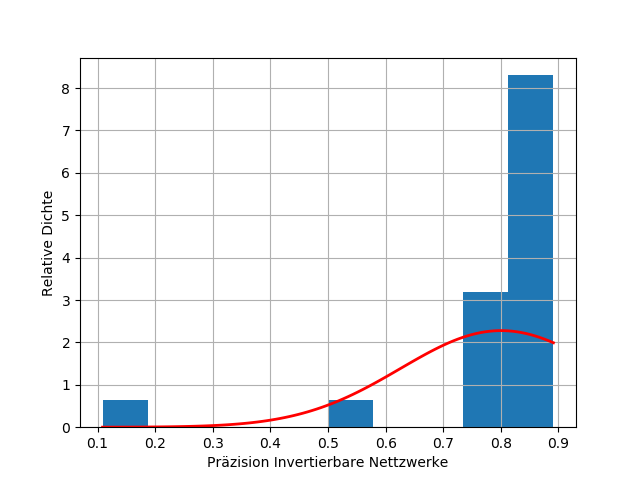
\includegraphics[width=\linewidth]{img/results/histogram_inverted_network_accuracy.png}
		\captionof{figure}{Präzision des komprimierten Neuronalen Neztes mehrere Matrizen}
		\label{fig:hist_inverted_network_accuracy}
	\end{Figure}
	
	\subsection{Invertierung mit Pseudoinvers}
	Auf den Bildern, welche durch die Invertierung des Neuronalen Netzes mit Hilfe des Pseudoinversen entstanden, ist nur Rauschen zu erkennen. In der Abbildung \ref{fig:dig_ideal_0_inverted} ist das errechnete Bild für den Vektor $ \begin{bmatrix}1 & 0 & 0 & 0 & 0 & 0 & 0 & 0 & 0 & 0 \end{bmatrix}^{T} $ zu sehen. Dies würde einer idealen Null entsprechen.
	\begin{Figure}
		\centering
		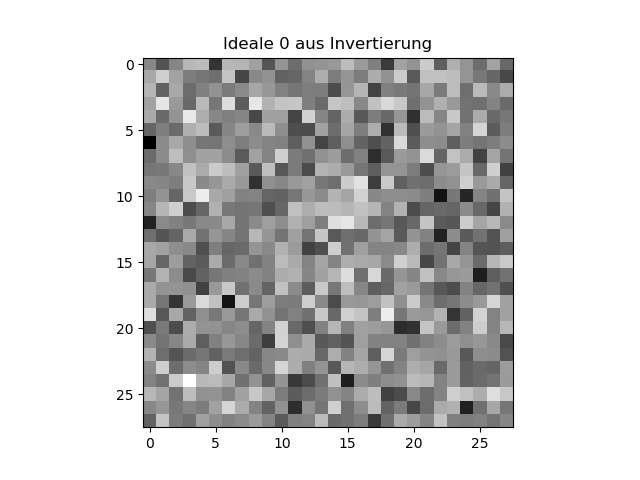
\includegraphics[width=\linewidth]{img/results/ideal_0_inverted.png}
		\captionof{figure}{Ideale 0 aus Invertierung}
		\label{fig:dig_ideal_0_inverted}
	\end{Figure}

	Das selbe Muster ist bei Abbildung \ref{fig:dig_interpolated_4_9_50_inverted} zu erkennen. Hier handelt es sich um ein Bild für eine Interpolation zwischen einer idealen vier und einer idealen neun. Der Winken für die Interpolation wurde so gewählt, dass sich der Vektor genau zwischen den beiden Werten befindet. Auch hier ist lediglich Rauschen zu erkennen.
	\begin{Figure}
		\centering
		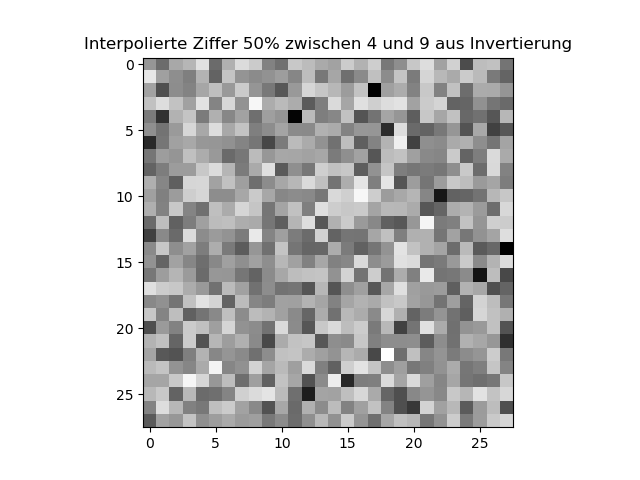
\includegraphics[width=\linewidth]{img/results/interpolated_4_9_50_inverted.png}
		\captionof{figure}{Interpolation von 4 und 9 durch Invertierung}
		\label{fig:dig_interpolated_4_9_50_inverted}
	\end{Figure}
	
	\subsection{Invertierung mit quadratischen Matrizen}
	Das Trainieren eines Neuronalen Netzes, welches nur quadratische Matrizen verwendet, erwies sich als äussert schwer. Die Trainingszeiten wuchsen stark an und die Resultate waren deutlich schlechter als die der Netze ohne quadratischen Matrizen. Der Abbildung \ref{fig:hist_squared_network_accuracy} kann entnommen werden, dass die meisten Netzwerke mit quadratischen Matrizen Trefferquoten von ungefähr 15\% erreichen.
	\begin{Figure}
		\centering
		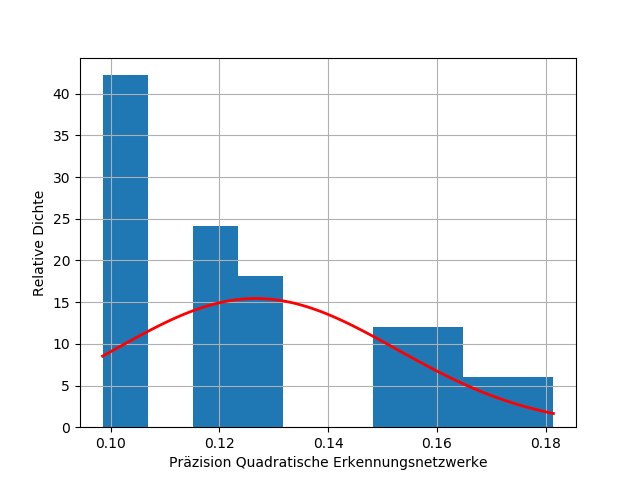
\includegraphics[width=\linewidth]{img/results/histogram_squared_network_accuracy.png}
		\captionof{figure}{Präzision des Neuronalen Neztes mit quadratischen Matrizen}
		\label{fig:hist_squared_network_accuracy}
	\end{Figure}

	Um zu sehen, ob sich mehr Aufwand in diese Richtung lohnt, wurden Tests für die Präzision beim Invertieren der Neuronalen Netzen mit quadratischen Matrizen gemacht. Die Resultate dazu sind im Kapitel \ref{sec:results_error_inverse} zu finden.
	\subsection{Fehler bei Gleitkommazahloperationen}
	\label{sec:results_error_inverse}
	Um zu bestimmen, wie sich die Rundungsfehler der Gleitkommazahlen auf Invertierung des Neuronalen Netzwerks auswirken, wurden verschiedene zufällig generierte Matrizen vor- und rückwärts durch das Neuronalen Netz gerechnet und der durchschnittliche Fehler pro Wert in der Matrix bestimmt. Die Matrizen wurden gewählt sodass $ M \in \mathbb{R}^{n \times n}, n \in [3, 9] $ und im Neuronalen Netz durch eine bis vier Schichten gerechnet. Die Resultate sind der Tabelle \ref{tbl:reverse_error} zu entnehmen. Daraus lässt sich erkennen, dass bei einer Matrix aus $ \mathbb{R}^{9 \times 9} $ bereits ein Netzwerk mit einer Schicht die Werte der Matrix im Schnitt die Werte im Bereich von $ 10^{0} $ verändert. Bei vier Schichten wird dieser Wert bereits bei einer Matrix aus $ \mathbb{R}^{6 \times 6} $ überschritten.
	\begin{table}[H]
		\centering
		\begin{tabular}{|l|r|r|r|r|}
			\hline
			 & 1 Layer & 2 Layers & 3 Layers & 4 Layers  \\ \hline
			$ \mathbb{R}^{3 \times 3} $ & 8.2e-15 & 3.8e-12 & 1.5e-08 & 1.6e-09 \\ \hline
			$ \mathbb{R}^{4 \times 4} $ & 1.6e-13 & 3.3e-10 & 3.35e-05 & 1.7e-04 \\ \hline
			$ \mathbb{R}^{5 \times 5} $ & 1.9e-10 & 5.0e-08 & 2.3e-06 & 6.1e-03 \\ \hline
			$ \mathbb{R}^{6 \times 6} $ & 1.0e-02 & 1.6e-02 & 3.4e-02 & 4.7e+00 \\ \hline
			$ \mathbb{R}^{7 \times 7} $ & 9.7e-02 & 2.3e-01 & 2.5e+00 & 1.3e+01 \\ \hline
			$ \mathbb{R}^{8 \times 8} $ & 4.5e-01 & 2.3e-01 & 6.2e+00 & 1.7e+01 \\ \hline
			$ \mathbb{R}^{9 \times 9} $ & 2.1e+00 & 1.6e+00 & 7.3e+00 & 1.9e+01 \\ \hline
		\end{tabular}
		\caption{Durchschnittlicher Fehler pro Wert nach Invertierung}
		\label{tbl:reverse_error}
	\end{table}	
	
	\subsection{Approximieren der Inputbilder}
	Bei der Approximation der Bilder wurde als Qualität der Fehler aus der Kreuzentropie zwischen dem erreichten Vektor und dem gewünschten Vektor für das zu generieren Bild verwendet. Hier lassen sich unterschiede für die Approximation der idealen Ziffern und der interpolierten Ziffern erkennen. In der Abbildung \ref{fig:hist_approximation_error_ideal} ist zu erkennen, dass für die idealen Ziffern der durchschnittliche Fehler bei 1.5 liegt, wobei es einige Ausreisser bei über 2.2 gibt.
	\begin{Figure}
		\centering
		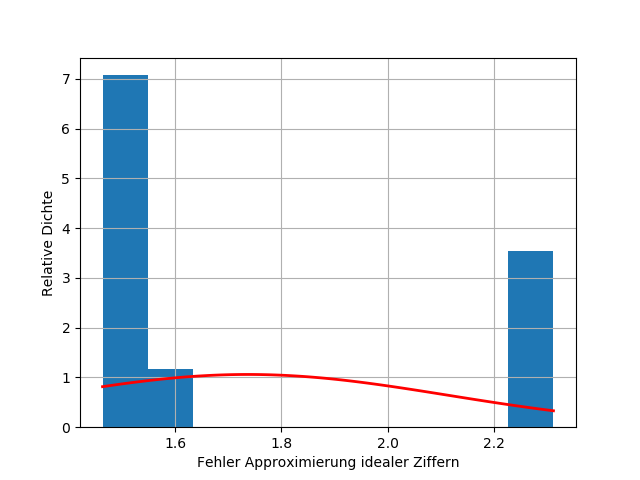
\includegraphics[width=\linewidth]{img/results/histogram_approximation_error_ideal.png}
		\captionof{figure}{Fehler bei Approximation idealer Ziffern}
		\label{fig:hist_approximation_error_ideal}
	\end{Figure}	
	
	In der Abbildung \ref{fig:hist_approximation_error_interpolation} ist zu sehen, dass der Fehler für die interpolierten Ziffern höher liegt als der der idealen Ziffern. Zu erkennen ist auch dass sich der Median in der Nähe von 2.2 erkennen lässt, was nahe an Fehlerwert der Ausreisser der idealen Ziffern ist.
	\begin{Figure}
		\centering
		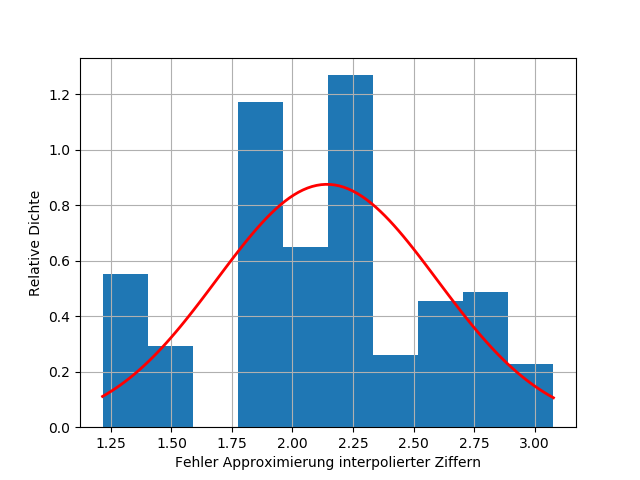
\includegraphics[width=\linewidth]{img/results/histogram_approximation_error_interpolation.png}
		\captionof{figure}{Fehler bei Approximation interpolierter Ziffern}
		\label{fig:hist_approximation_error_interpolation}
	\end{Figure}
	
	Die generierten Bilder sind auch hier nur Rauschen. Auch bei den tiefen Fehlerwerten der idealen Ziffern ist keine Struktur zu erkennen. In der Abbildung \ref{fig:dig_ideal_7_approximated} ist das approximierte Bild für eine ideale 7 zu sehen.
	\begin{Figure}
		\centering
		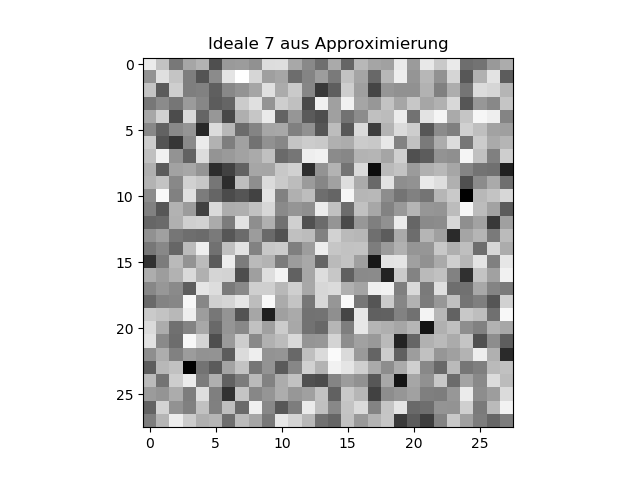
\includegraphics[width=\linewidth]{img/results/ideal_7_approximated.png}
		\captionof{figure}{Ideale 7 durch Approximierung}
		\label{fig:dig_ideal_7_approximated}
	\end{Figure}
	
	In einem letzten Versuch wurden für die Approximation anstelle von zufällig generierten Matrizen Bilder aus dem Trainingssatz verwendet. Dies führte dazu, dass die Approximation die Inputmatrix nicht veränderte, auch wenn eine andere Ziffer als Ziel der Approximation angegeben wurde.

\end{document}